
% --------------------------

% Figure
\begin{figure}[]
\begin{center}
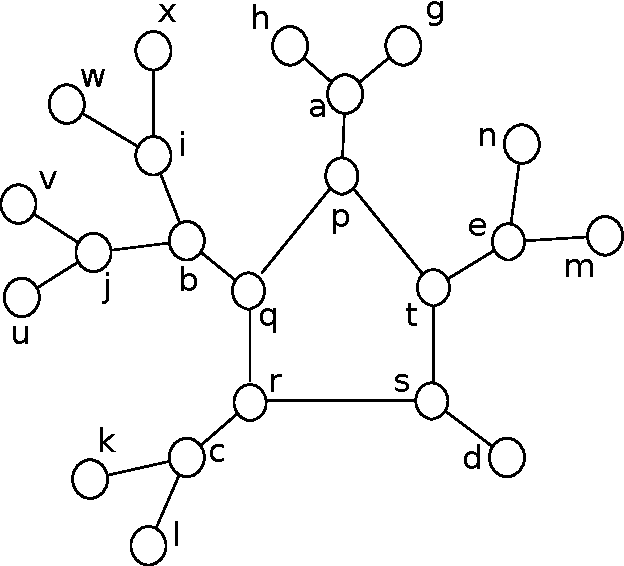
\includegraphics[scale=0.4]{pent}
\caption{Pentagon $pqrst$}
\label{fig:pent}
\end{center}
\end{figure}

% --------------------------

% Table
\begin{table}
\centering
\begin{tabular}{| c | c |}
\hline
{\bf item 1} & {\bf item 2} \\ \hline
%
abcde & 5 \\ \hline
%
pqrst & 4 \\ \hline
\end{tabular}
\caption{A sample table}
\label{table:1}
\end{table}

% --------------------------

You should cite papers in the following manner:
Bayliss et al.~\cite{gyrophone} gave an iterative method for Helmholtz equation etc.
Similar work has been done in \cite{walnut, goespin}.
